\chapter[Supporting Information for ``Tracking Rodinia in the Neoproterozoic: new paleomagnetic constraint from the Jacobsville Formation"][Supporting Information--Jacobsville Formation]{Supporting Information for ``Tracking Rodinia in the Neoproterozoic: new paleomagnetic constraint from the Jacobsville Formation"}

\begin{figure}
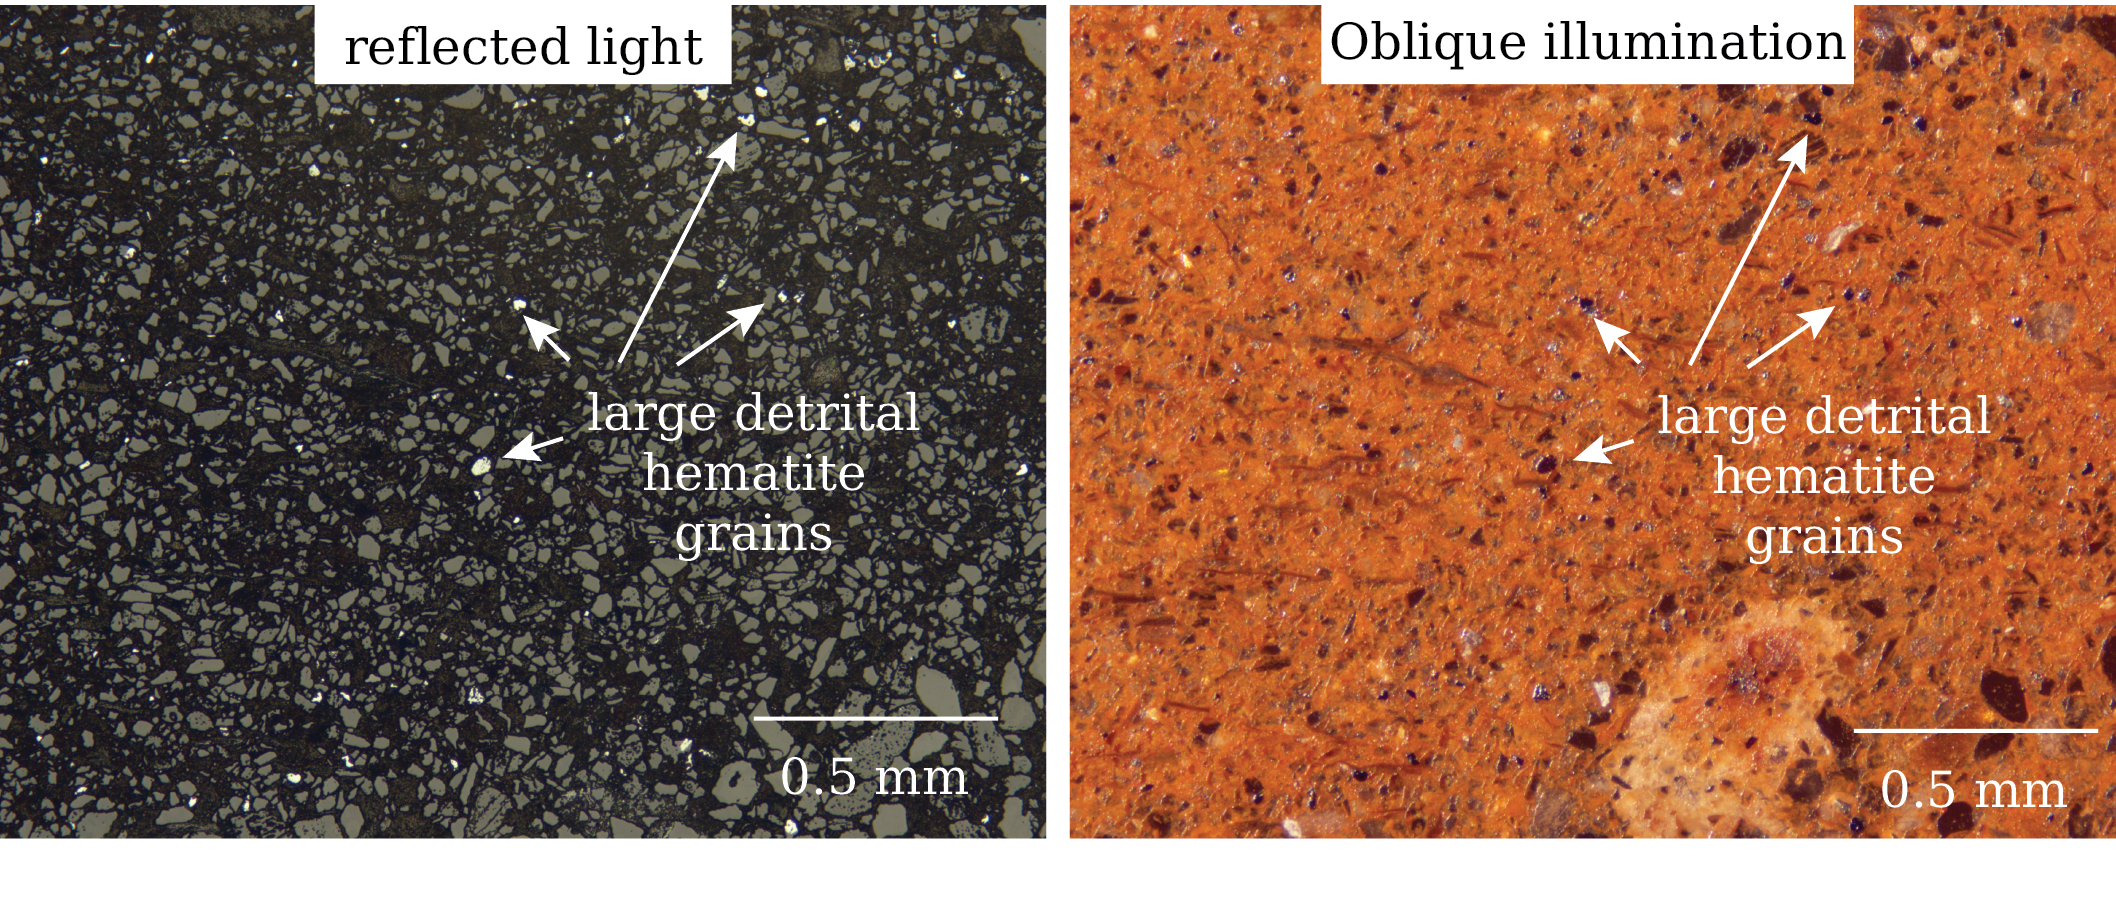
\includegraphics[width=0.9\textwidth]{figure/Zhang2024a/SI_petrography.png}
\caption[Petrographic images of fine-grained sandstone facies of the Jacobsville Formation]{Side-by-side reflected light and oblique illumination images of a thin section of the same field of view of sample NW2-7 collected from Natural Wall ravine. The white arrows point towards examples of large sub-millimeter-scale detrital hematite grains that have bright reflectance under reflected light. Almost all subangular grains in grey color in the reflected image are quartz grains. The red color in the oblique illumination image is a result of diffuse reflectance of pigmentary hematite grains that often coat the boundaries of detrital grains. }
\label{fig:SI_petrography}
\end{figure}

\begin{figure}
\centering
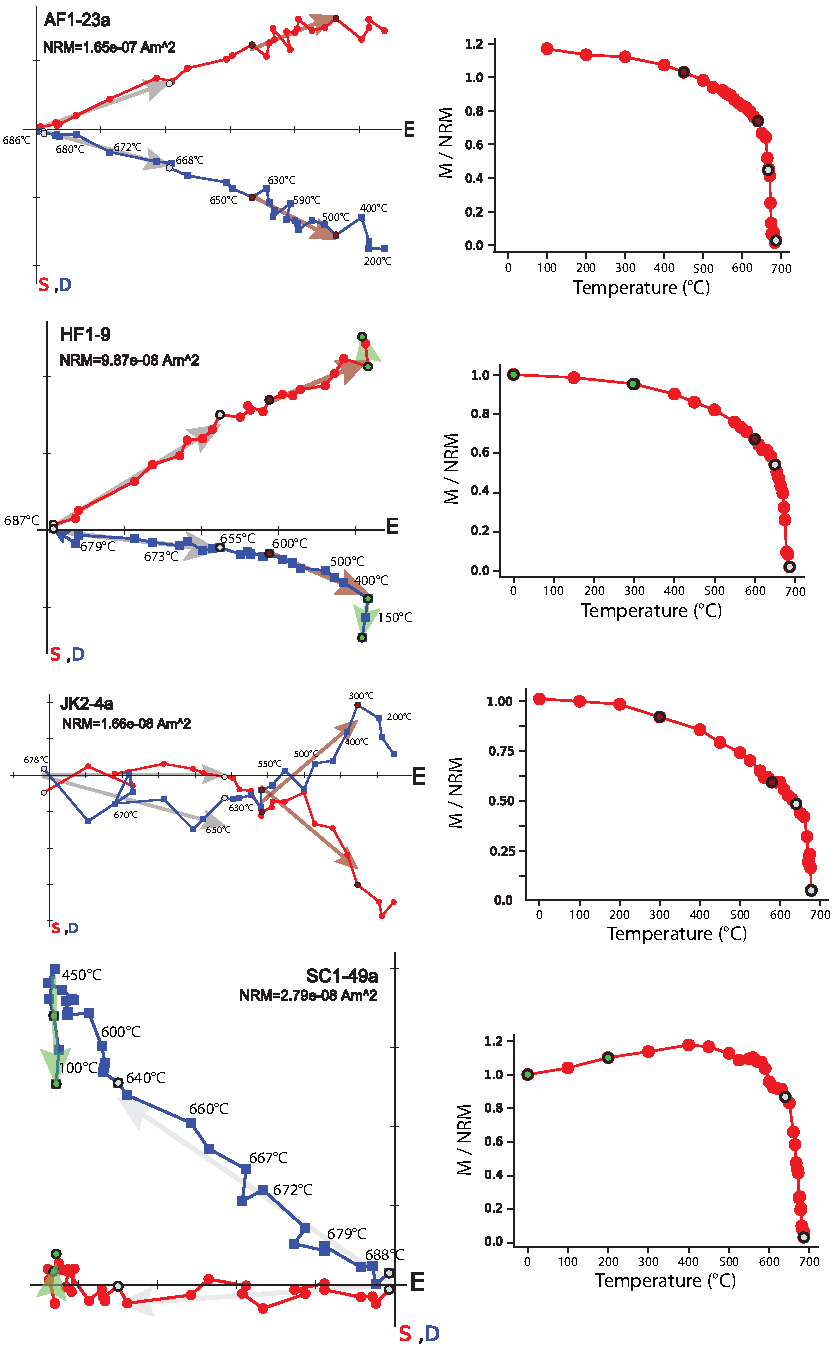
\includegraphics[width=0.6\textwidth]{figure/Zhang2024a/SI_orthogonal.pdf}
\caption[Representative orthogonal vector diagrams of demagnetization experiments for specimens from different stratigraphic sections of the Jacobsville Formation]{Representative orthogonal vector diagrams of demagnetization experiments for specimens from different stratigraphic sections of this study. An overprint component subparallel to the present day field direction in the study area is typically minimally present in siltstone to very fine-grained sandstone facies. This component shown in light green can be fit with a least-squares line in fine-grained facies. After the removal of the low-temperature component, a mid-temperature component typically unblocks through a wide range of temperature steps by up to $\sim$650\textdegree C. Finally, an origin-trending component with typically a shallower inclination than that of the mid-temperature component sharply unblocks through heating with smaller temperature intervals up toward the N\'eel temperature of hematite ($\sim$690\textdegree C). AF-Agate Falls section; HF-Hungarian side falls section near Dover Creek; JK-Hammel Creek section; SC-Snake Creek tributary section. M-magnetic moment; NRM-natural remanent magnetic moment. All diagrams are shown in tilt-corrected coordinates.}
\label{fig:SI_orthogonal}
\end{figure}

\begin{figure}
\centering
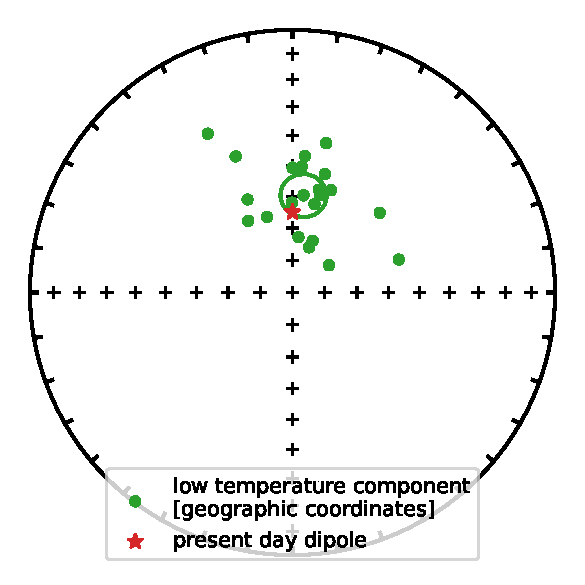
\includegraphics[width=0.5\textwidth]{figure/Zhang2024a/Jacobsville_pdf_directions.pdf}
\caption[Jacobsville Formation present day local field component]{Jacobsville present day local field directions. This present day overprint component is typically removed by $\sim$300\textdegree C.}
\label{fig:Jacobsville_pdf}
\end{figure}

\begin{figure}
\centering
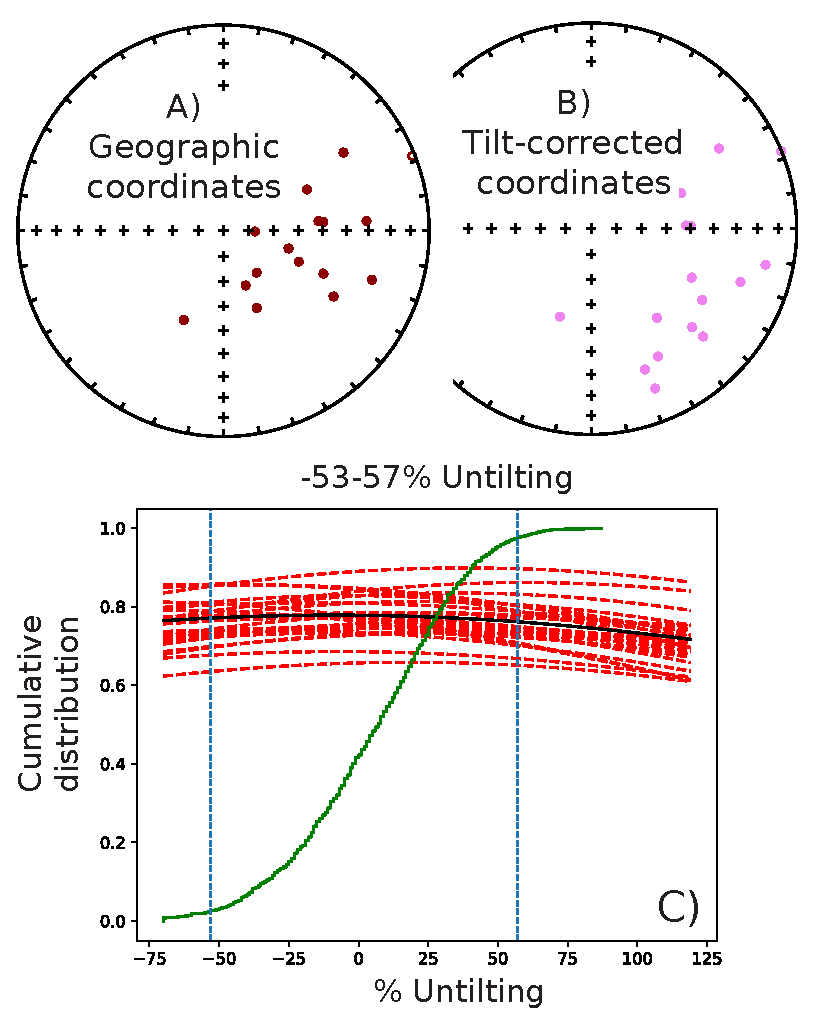
\includegraphics[width=0.9\textwidth]{figure/Zhang2024a/SI_hct_fold_test.pdf}
\caption[Paleomagnetic fold test at the Snake Creek tributary of the Jacobsville Formation]{Bootstrap paleomagnetic fold test \citep{Tauxe1994a} of the chemical remanent magnetization directions recorded by specimens from the nearly horizontal beds and moderately tilted beds at the Snake Creek tributary. Complete unfolding does not lie within the 95\% confidence limits of the test, consistent with the magnetization having been acquired syn- to post-folding.}
\label{fig:Jacobsville_hct_fold_test}
\end{figure}

\begin{figure}
\centering
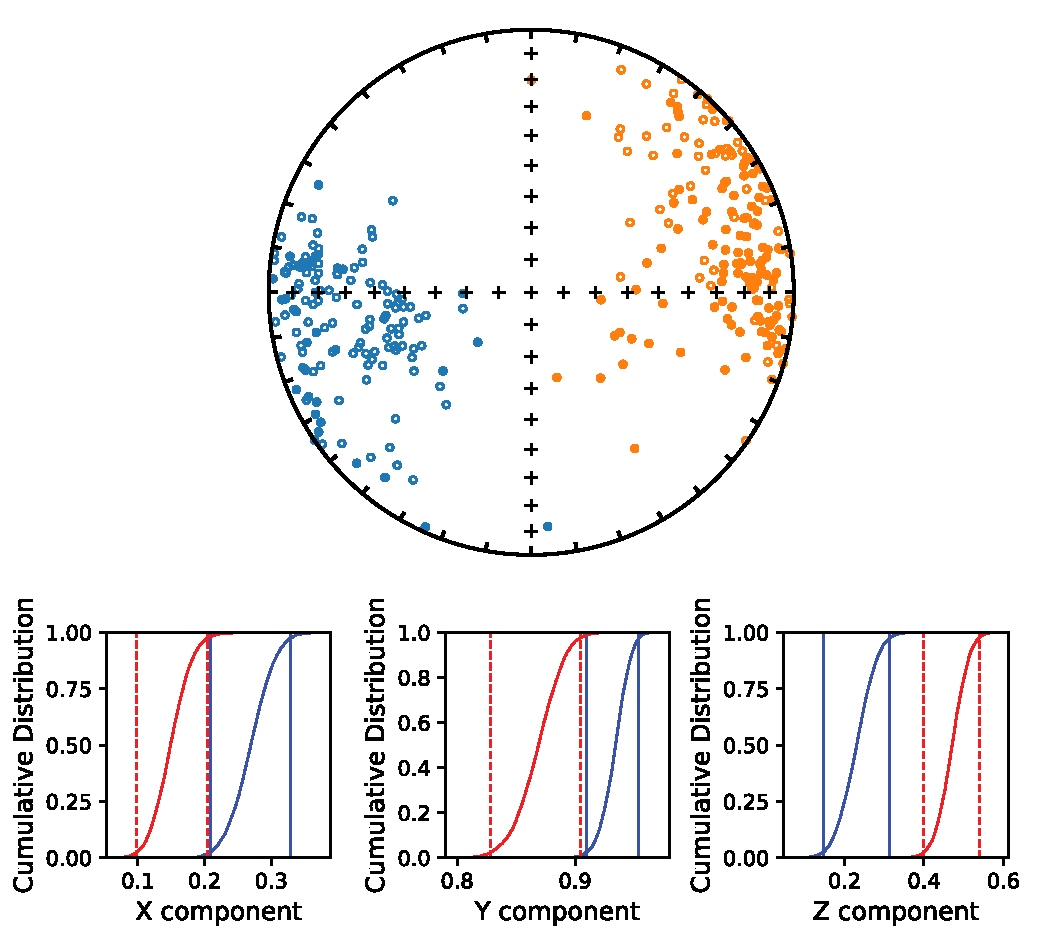
\includegraphics[width=0.9\textwidth]{figure/Zhang2024a/SI_reversal_test.pdf}
\caption[Paleomagnetic reversal test of the Jacobsville detrital remanence]{Jacobsville detrital remanence directions showing dual polarities plotted on an equal area stereonet plot. The directions do not pass a reversal test of \cite{McFadden1990a} as the angle between the mean directions is 15.9\textdegree\, larger than the critical angle of 7.5\textdegree. The directions also do not pass the bootstrap reversal test of \cite{Tauxe1991a}. }
\label{fig:Jacobsville_reversal_test}
\end{figure}

\begin{figure}
\centering
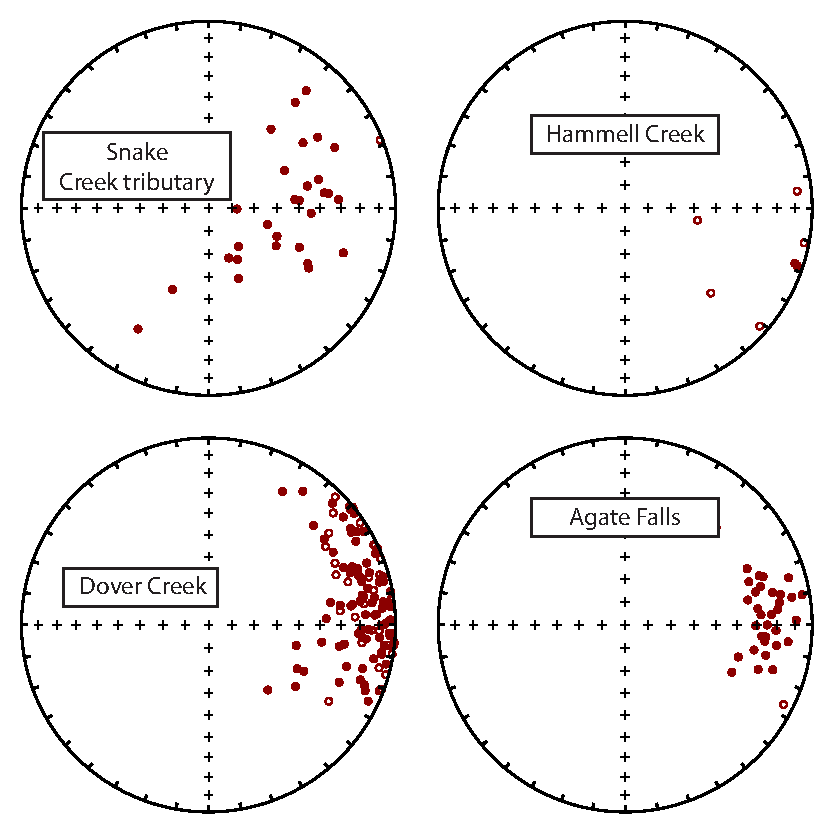
\includegraphics[width=0.9\textwidth]{figure/Zhang2024a/SI_hct.pdf}
\caption[Jacobsville Formation chemical remanence directions]{Jacobsville chemical remanence magnetization directions plotted by section. Samples collected from the Natural Wall section do not have interpretable chemical remanence component that can be fit with least-squares lines. All directions are plotted in geographic coordinates.}
\label{fig:Jacobsville_CRM}
\end{figure}

\begin{figure}
\centering
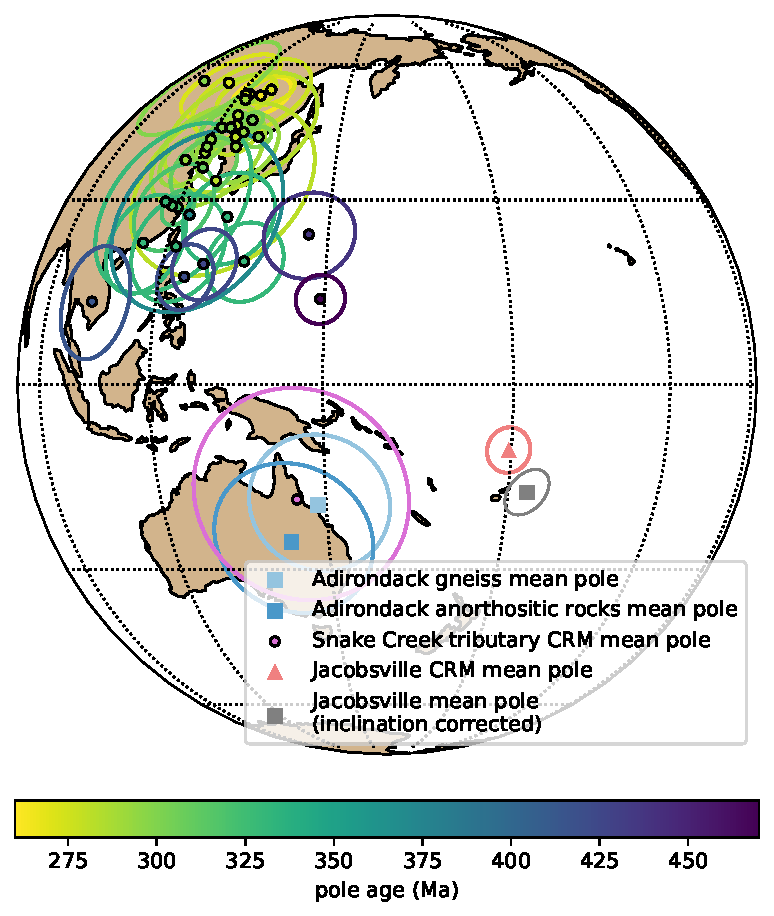
\includegraphics[width=0.75\textwidth]{figure/Zhang2024a/SI_Jacobsville_vs_Appalachian_poles.pdf}
\caption[Jacobsville detrital remanence pole position in context of Laurentia's paleomagnetic poles during Appalachian orogeny (ca. 460-260 Ma) as compiled in \cite{Torsvik2012a}]{Jacobsville detrital remanence Kent mean pole position and chemical remanence Fisher mean pole position (in geographic coordinates) plotted in context of Laurentia's paleomagnetic poles during Appalachian orogeny (ca. 460-260 Ma) as compiled in \cite{Torsvik2012a}. The mean chemical remanence pole position from the Snake Creek tributary section is plotted in context of the ca. 970-960 Ma poles developed by \cite{Brown2012a} from the Adirondack Highlands of the Grenville orogen. That this chemical remanence component failed a fold test (Figure \ref{fig:Jacobsville_hct_fold_test}) and yields a pole position that overlaps with the Grenville poles are consistent with the interpretation that the chemical remanence of the Jacobsville Formation at this locality was acquired  during the early Neoproterozoic, soon after Jacobsville deposition and deformation. That the Jacobsville DRM and CRM mean poles are distinct and far away from any of Laurentia's mid- to late-Paleozoic poles supports the interpretation that the Jacobsville detrital remanence magnetization was acquired during the Rigolet phase of the Grenvillian orogeny and the chemical remanence overprint was likely acquired soon after deposition as discussed in detail in the manuscript.}
\label{fig:Jacobsville_Appalachian}
\end{figure}

\begin{figure}
\centering
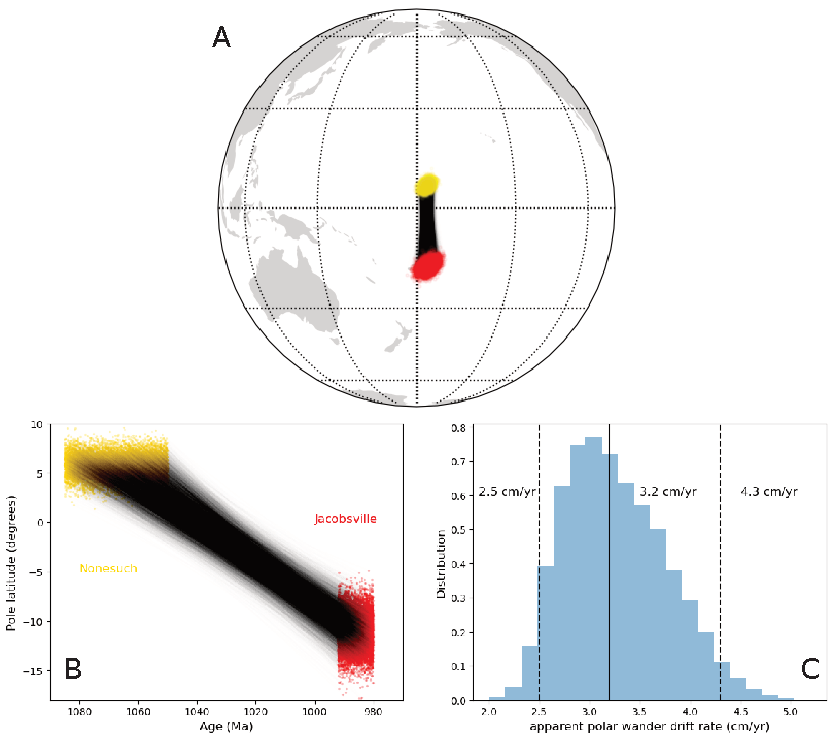
\includegraphics[width=0.9\textwidth]{figure/Zhang2024a/SI_Jacobsville_Nonesuch_rate.pdf}
\caption[Monte Carlo simulations of apparent polar wander rates implied by paleomagnetic and geochronologic data between the Nonesuch Formation and the Jacobsville Formation]{Monte Carlo simulations of apparent polar wander rates implied by paleomagnetic and geochronologic data between the Nonesuch Formation and the Jacobsville Formation. (A) The gold and red points are 10,000 simulated Kent distribution mean paleomagnetic poles for the Nonesuch Formation and Jacobsville Formation, respectively. The simulated poles are connected by gray lines which represent the apparent polar wander great circle paths. (B) The points color-coded in the same way as in (A) show the simulated paleomagnetic pole latitudes plotted against their simulated pole ages using uniform distributions. The points are connected by gray lines which represent the simulated pole latitudinal motion. The histogram on the right shows all 10,000 of the simulated rates that yield the labeled 2.5 percentile value of 2.5 cm/yr, median value of 3.2 cm/yr and 97.5 percentile value of 4.3 cm/yr.}
\label{fig:Jacobsville_Nonesuch_rate}
\end{figure}

\begin{sidewaystable}
\tiny
\caption[Compilation of Laurentian paleomagnetic poles]{\scriptsize Compilation of up-to-date Keweenawan Track paleomagnetic poles and ca. 780-720 Ma Laurentian paleomagnetic poles. }
\begin{tabular}{p{4cm}lllp{4cm}p{1.3cm}p{1.2cm}p{1.2cm}p{4cm}}

\hline
\multicolumn{9}{c}{Compilation of Fisher mean paleomagnetic poles}                                                                                                                                                                                        \\ \hline
Pole                                                       & Pole lat & Pole lon & A95  & Pole reference                                                         & AgeNominal & AgeLower & AgeUpper & Age reference                                       \\
Osler reverse (lower)                                      & 40.9     & 218.6    & 4.8  & \cite{Swanson-Hysell2014a}                                           & 1108       & 1105.15  & 1110     & \cite{Davis1985a, Swanson-Hysell2019a}               \\
Osler reverse (upper)                                      & 42.3     & 203.4    & 3.7  & \cite{Halls1974a, Davis1985a, Swanson-Hysell2014a} & 1105.15    & 1104.82  & 1105.48  & \cite{Swanson-Hysell2019a}                       \\
Mamainse lower reversed 1                                  & 49.5     & 227      & 5.3  & \cite{Swanson-Hysell2014b}                                           & 1109       & 1106     & 1112     & As discussed in \cite{Swanson-Hysell2019a}         \\
Mamainse lower reversed 2                                  & 37.5     & 205.2    & 4.5  & \cite{Swanson-Hysell2014b}                                                  & 1105       & 1100.4   & 1109     & \cite{Swanson-Hysell2014b}                              \\
Mamainse lower normal and upper reversed                   & 36.1     & 189.7    & 4.9  & \cite{Swanson-Hysell2014b}                                                  & 1100.36    & 1100.1   & 1100.61  & \cite{Swanson-Hysell2014b}                               \\
Mamainse upper normal                                      & 31.2     & 183.2    & 2.5  & \cite{Swanson-Hysell2014b}                                                  & 1094       & 1090     & 1100     & As discussed in S\cite{Swanson-Hysell2019a}            \\
Grand Portage Basalts                                      & 46       & 201.7    & 6.8  & \cite{Books1968a, Tauxe2009a}                                    & 1106       & 1105.28  & 1108     & \cite{Swanson-Hysell2019a}                         \\
North Shore Volcanic Group (upper NE   sequence)           & 31.1     & 181.7    & 4.2  & \cite{Books1972a, Tauxe2009a}                                    & 1095       & 1092     & 1098     & \cite{Davis1997a, Fairchild2017a}       \\
North Shore Volcanic Group (upper SW   sequence)           & 36.9     & 179.3    & 2.1  & \cite{Tauxe2009a, Swanson-Hysell2019a}                   & 1096.18    & 1093.94  & 1096.75  & \cite{Swanson-Hysell2019a}                        \\
Schroeder Lutsen Basalts                                   & 28.3     & 187.6    & 2.5  & \cite{Books1972a, Tauxe2009a, Fairchild2017a}            & 1090       & 1085     & 1091.5   & \cite{Fairchild2017a}                               \\
Portage Lake Volcanics                                     & 27.5     & 182.5    & 2.3  & \cite{Books1972a, Hnat2006a}                                         & 1092.51    & 1091.59  & 1093.37  & \cite{Swanson-Hysell2019a}                    \\
Lake Shore Traps                                           & 22.2     & 180.8    & 4.5  & \cite{Diehl1994a}                                                     & 1085.47    & 1084     & 1091     & \cite{Fairchild2017a, Swanson-Hysell2019a}    \\
Siemens Creek Volcanics                                    & 45.8     & 214      & 9.2  & \cite{Palmer1986a}                                                 & 1108       & 1105     & 1111     & \cite{Davis1997a}                               \\
Michipicoten Island Formation                              & 17       & 174.7    & 4.4  & \cite{Palmer1987a, Fairchild2017a}                        & 1083.95    & 1083.52  & 1084.39  & \cite{Fairchild2017a}                           \\
Freda Formation                                            & 2.2      & 179      & 4.2  & \cite{Henry1977a}                                                     & 1070       & 1060     & 1083.5   & As discussed in \cite{Swanson-Hysell2019a}            \\
Haliburton Intrusions                                      & -36.2    & 141.7    & 6.0  & \cite{Buchan1976a}                          & 1015       & 1000     & 1030     & \cite{Warnock2000a}                                          \\
Adirondack Highlands gneiss                                & -19      & 148.7    & 11.2 & \cite{Brown2012a}                                                &            &          &          &                                                     \\
Adirondack Highlands anorthositic rocks                    & -25.2    & 143.4    & 12.9 & \cite{Brown2012a}                                                &            &          &          &                                                     \\
Adirondack Highlands granites                              & -28.5    & 131.7    & 7.1  & \cite{Brown2012a}                                                &            &          &          &                                                     \\
Franklin large igneous province   Victoria/Mainland/Baffin & 6.7      & 162.1    & 3    & \cite{Denyszyn2009a}                                                   & 716.33     & 715.79   & 716.87   &                                                     \\
Combo Carbon Butte–Awatubi                                 & 14.2     & 163.8    & 3.5  & \cite{Eyster2019a}                                                   & 751        & 743.4    & 758.6    &                                                     \\
Carbon Canyon                                              & -0.5     & 166      & 9.7  & compilation by \cite{Eyster2019a}                                    & 757        & 750.2    & 763.8    &                                                     \\
UMG Group 3                                                & 4.9      & 160.6    & 3.2  & compilation by \cite{Eyster2019a}                                    & 755        &          &          & As discussed in \cite{Eyster2019a}                \\
Nankoweap                                                  & -10      & 163      & 4.9  & \cite{Weil2003a}                                                     & 782        &          &          & As discussed in Eyster et al., 2020                 \\
UMG Group 2                                                & -5.8     & 158.7    & 2.7  & compilation by \cite{Eyster2019a}                                    & 760        &          &          & As discussed in Eyster et al., 2021                 \\
UMG Group 1                                                & 3        & 163.5    & 3.2  & compilation by \cite{Eyster2019a}                                    & 766        &          &          & As discussed in Eyster et al., 2022                 \\
Gunbarrel mean                                             & 9.1      & 138.2    & 11.7 & \cite{Eyster2019a}                                                   & 774.93     & 774.39   & 775.47   &                                                    
\end{tabular}
\label{tab:pole_compilation}
\end{sidewaystable}

\clearpage

\begin{sidewaystable}
\begin{scriptsize}
\begin{tabular}{p{1.5cm}p{1cm}p{1cm}p{1cm}p{1cm}p{1cm}p{1cm}p{1cm}p{1cm}p{1cm}p{1cm}p{1cm}p{1cm}p{2cm}}
\hline
\multicolumn{14}{c}{Compilation of Kent mean paleomagnetic poles}                                                                                                                                                                                           \\ \hline 
Pole                  & Pole lat & Pole lon & Major axis lat & Major axis lon & Major axis magnitude & Minor axis lat & Minor axis lon & Minor axis magnitude & Pole reference         & Age Nominal & Age Lower & Age Upper & Age reference                                       \\
Nonesuch Formation    & 6.6      & 182.9    & 27.6           & 280.2          & 2.8                  & 41.6           & 87             & 2                    & \cite{Slotznick2023a} & 1080       & 1070     & 1083.5   & As discussed in \cite{Swanson-Hysell2019a}         \\
Jacobsville Formation & 16.9    & 183.4    & 45.2           & 255.5          & 4.1                    & 39.9           & 108.1          & 3.1                  & this study             & 990        & 985      & 992     & \cite{Hodgin2022a}; as discussed in the manuscript
\end{tabular}
\end{scriptsize}
\end{sidewaystable}

\clearpage


